\documentclass{standalone}

\usepackage{tikz}

\begin{document}

\newcommand{\PolygonInit}{
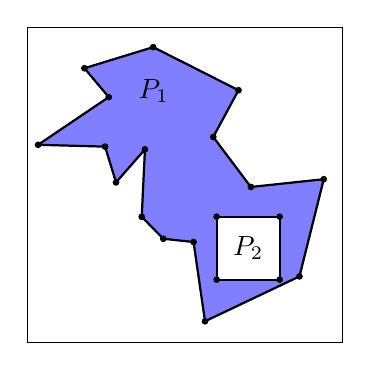
\begin{tikzpicture}[scale=4]
\coordinate (A) at (0.1802,0.8712);
\coordinate (B) at (0.2573,0.7795);
\coordinate (C) at (0.0331,0.6281);
\coordinate (D) at (0.2457,0.6223);
\coordinate (E) at (0.2806,0.5088);
\coordinate (F) at (0.3723,0.6136);
\coordinate (G) at (0.3621,0.3996);
\coordinate (H) at (0.4306,0.3297);
\coordinate (I) at (0.5266,0.3195);
\coordinate (J) at (0.5630,0.0677);
\coordinate (K) at (0.8629,0.2103);
\coordinate (L) at (0.9401,0.5189);
\coordinate (M) at (0.7086,0.4942);
\coordinate (N) at (0.5892,0.6529);
\coordinate (O) at (0.6693,0.8014);
\coordinate (P) at (0.3985,0.9382);

\coordinate (Q) at (0.6,0.4);
\coordinate (R) at (0.6,0.2);
\coordinate (S) at (0.8,0.2);
\coordinate (T) at (0.8,0.4);

\fill[blue, fill opacity = 0.5] (A)--(B)--(C)--(D)--(E)--(F)--(G)--(H)--(I)--(J)--(K)--(L)--(M)--(N)--(O)--(P)--cycle;
\draw[thick] (A)--(B)--(C)--(D)--(E)--(F)--(G)--(H)--(I)--(J)--(K)--(L)--(M)--(N)--(O)--(P)--cycle;

\fill[white] (Q)--(R)--(S)--(T)--cycle;
\draw[thick] (Q)--(R)--(S)--(T)--cycle;

\node at (0.4,0.8) {$P_1$};
\node at (0.7,0.3) {$P_2$};

\foreach \pt in {A,B,C,D,E,F,G,H,I,J,K,L,M,N,O,P,Q,R,S,T}{
	\draw[fill=black] (\pt) circle (0.25pt);
}
\useasboundingbox (0,0) rectangle (1,1);
\draw (0,0) rectangle (1,1);
\end{tikzpicture}
}

\newcommand{\ConvexHull}{
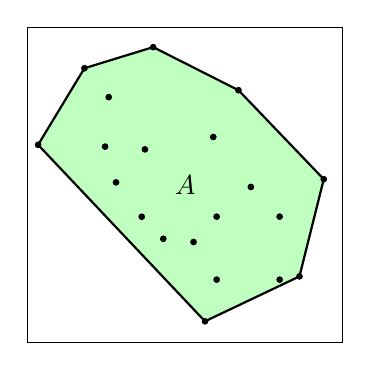
\begin{tikzpicture}[scale=4]
\useasboundingbox (0,0) rectangle (1,1);
\coordinate (A) at (0.1802,0.8712);
\coordinate (B) at (0.2573,0.7795);
\coordinate (C) at (0.0331,0.6281);
\coordinate (D) at (0.2457,0.6223);
\coordinate (E) at (0.2806,0.5088);
\coordinate (F) at (0.3723,0.6136);
\coordinate (G) at (0.3621,0.3996);
\coordinate (H) at (0.4306,0.3297);
\coordinate (I) at (0.5266,0.3195);
\coordinate (J) at (0.5630,0.0677);
\coordinate (K) at (0.8629,0.2103);
\coordinate (L) at (0.9401,0.5189);
\coordinate (M) at (0.7086,0.4942);
\coordinate (N) at (0.5892,0.6529);
\coordinate (O) at (0.6693,0.8014);
\coordinate (P) at (0.3985,0.9382);

\coordinate (Q) at (0.6,0.4);
\coordinate (R) at (0.6,0.2);
\coordinate (S) at (0.8,0.2);
\coordinate (T) at (0.8,0.4);

\fill[green, fill opacity = 0.25] (A)--(C)--(J)--(K)--(L)--(O)--(P)--cycle;
\draw[thick] (A)--(C)--(J)--(K)--(L)--(O)--(P)--cycle;

\node at (0.5,0.5) {$A$};

\foreach \pt in {A,B,C,D,E,F,G,H,I,J,K,L,M,N,O,P,Q,R,S,T}{
	\draw[fill=black] (\pt) circle (0.25pt);
}

\draw (0,0) rectangle (1,1);
\end{tikzpicture}
}

\newcommand{\Trous}{
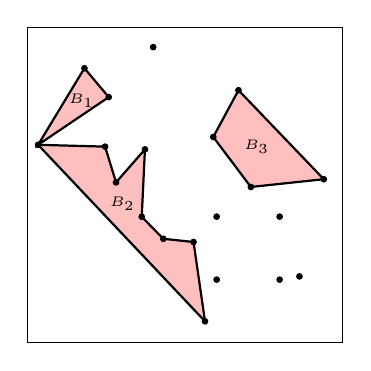
\begin{tikzpicture}[scale = 4]
\useasboundingbox (0,0) rectangle (1,1);

\coordinate (A) at (0.1802,0.8712);
\coordinate (B) at (0.2573,0.7795);
\coordinate (C) at (0.0331,0.6281);
\coordinate (D) at (0.2457,0.6223);
\coordinate (E) at (0.2806,0.5088);
\coordinate (F) at (0.3723,0.6136);
\coordinate (G) at (0.3621,0.3996);
\coordinate (H) at (0.4306,0.3297);
\coordinate (I) at (0.5266,0.3195);
\coordinate (J) at (0.5630,0.0677);
\coordinate (K) at (0.8629,0.2103);
\coordinate (L) at (0.9401,0.5189);
\coordinate (M) at (0.7086,0.4942);
\coordinate (N) at (0.5892,0.6529);
\coordinate (O) at (0.6693,0.8014);
\coordinate (P) at (0.3985,0.9382);

\coordinate (Q) at (0.6,0.4);
\coordinate (R) at (0.6,0.2);
\coordinate (S) at (0.8,0.2);
\coordinate (T) at (0.8,0.4);

% \fill[blue, fill opacity = 0.5] (A)--(B)--(C)--(D)--(E)--(F)--(G)--(H)--(I)--(J)--(K)--(L)--(M)--(N)--(O)--(P)--cycle;
% \draw[thick] (A)--(B)--(C)--(D)--(E)--(F)--(G)--(H)--(I)--(J)--(K)--(L)--(M)--(N)--(O)--(P)--cycle;

\fill[red, fill opacity = 0.25] (A)--(B)--(C)--cycle;
\draw[thick] (A)--(B)--(C)--cycle;

\fill[red, fill opacity = 0.25] (C)--(D)--(E)--(F)--(G)--(H)--(I)--(J)--cycle;
\draw[thick] (C)--(D)--(E)--(F)--(G)--(H)--(I)--(J)--cycle;

\fill[red, fill opacity = 0.25] (L)--(M)--(N)--(O)--cycle;
\draw[thick] (L)--(M)--(N)--(O)--cycle;

% \fill[white] (Q)--(R)--(S)--(T)--cycle;
% \draw[thick] (Q)--(R)--(S)--(T)--cycle;

\node at (0.1709,0.7677) {\tiny $B_1$};
\node at (0.3009,0.4416) {\tiny $B_2$};
\node at (0.7272,0.6228) {\tiny $B_3$};
% \node at (0.7,0.3) {$P_2$};

\foreach \pt in {A,B,C,D,E,F,G,H,I,J,K,L,M,N,O,P,Q,R,S,T}{
	\draw[fill=black] (\pt) circle (0.25pt);
}
\draw (0,0) rectangle (1,1);
\end{tikzpicture}
}

\begin{tikzpicture}

\node (PolygonInit){\PolygonInit};

\node[right of=PolygonInit, xshift = 1.5cm] (Egalite){$=$};

\node[right of=Egalite, xshift = 1.5cm] (ConvexHull) {\ConvexHull};

\node[right of=ConvexHull, xshift = 1.5cm] (Soustraction){$-$};

\node[right of=Soustraction, xshift = 1.5cm] (Trous) {\Trous};

\end{tikzpicture}


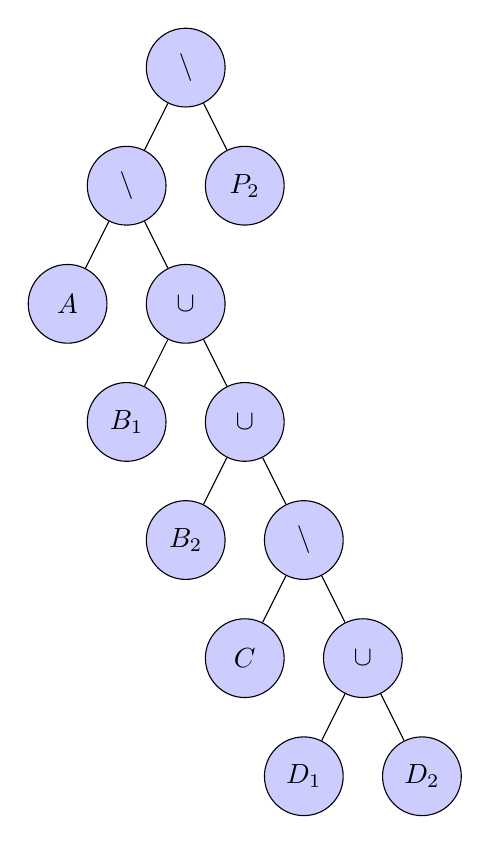
\begin{tikzpicture}[
mystyle/.style={draw, circle, minimum size = 1cm, fill = blue!20}
]
\node[mystyle] {$\setminus$}
	child {node[mystyle] {$\setminus$}
		child {node[mystyle] {$A$}}
		child {node[mystyle] {$\cup$}
    	child {node[mystyle] {$B_1$}}
    	child {node[mystyle] {$\cup$}
    		child {node[mystyle] {$B_2$}}
    		child {node[mystyle] {$\setminus$}
    			child {node[mystyle] {$C$}}
    			child {node[mystyle] {$\cup$}
    				child {node[mystyle] {$D_1$}}
    				child {node[mystyle] {$D_2$}}
    			}
    		}
    	}
    }
	}
    child {node[mystyle] {$P_2$}};
\end{tikzpicture}


\begin{tikzpicture}[
oper/.style={draw, circle, minimum size = 1cm},
drawing/.style={rectangle}
]
\node[oper] {$\setminus$}
child {node[drawing,yshift=-2cm,xshift=-1.5cm] {\ConvexHull}}
child {node[drawing,yshift=-2cm,xshift=1.5cm] {\Trous}}
;
\end{tikzpicture}

\end{document}